\section{Opnåede erfaringer}
\label{ch:OpXP}
\subsection{Generelt}
Gruppen har fra start ville uddelegere opgaver og ansvar for at lette arbejdsprocessen. Systemet blev derfor opdelt i moduler med en ansvarlig tilknyttet. Modulerne blev uddelt efter interesse. Dette har været en rigtig god løsning for flere af gruppens medlemmer tidligere, men i dette forløb har det vist sig også at være en hæmsko. Det fælles projektarbejde blev hurtigt fem personer, der sad med hvert deres lille område af projektet. Den interne kommunikation udeblev, og sparringen blev mangelfuld på grund af manglende indsigt i hvad de resterende gruppemedlemmer lavede.

Gruppen har i dette projekt bestået af 5 elektronik ingeniørstuderende. Dette har skabt nogle problemer med hensyn til programmeringsdele af projektet. Gruppen har dog været god til at søge hjælp til problematiske opgaver, hvilket har gjort at programmeringstunge moduler er blevet implementeret korrekt.\\

\subsection{Udvikling af hældningssensor}
Vi har startede med at udvikle på en prototype af en libellesensor vist på \textit{Figur~\ref{fig:libelle}}.
\begin{figure}[hbpt]
\centering
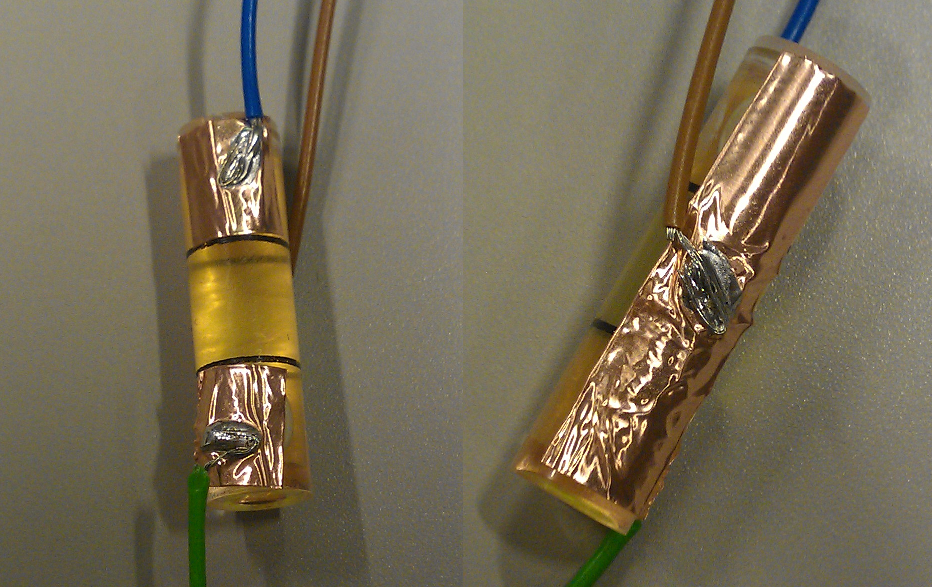
\includegraphics[width=0.5\textwidth]{billeder/libellesensor1}
\caption{henning}
\label{fig:libelle}
\end{figure}
Vi kom frem til at den har en capacitet på omkring $1*10^{-15}[F]$. Det gør det praktisk umuligt at anvende da vores filter så har en alt for stor cutoff frekvens liggende over 3.0 MHz. Den høje frekvens giver en stor selvinduktion i vores ledning. Samtidig kan vi ikke lave sinus med denne frekvens med PSoC'en. Dette gjorde at vi måtte finde en anden løsning.\\
Næste prototype bestod af et potmeter og et pendul. Dog havde potmeteret en for stor friktionsmodstand, der gjorde det upræcist i forhold til vores krav.\\
Vi har gennem et tredje semestersfag fundet ud af at PSoC'en indeholder et accelerometer. Vi valgte så at lave en prototype med det. Dette viste sig at være en god løsning.

\subsection{Metoder}
Gruppen var opsatte på at have læst review på projektets dokumentation, men de adspurgte grupper havde ingen interesse i at lave review udvekslinger. Dette har ført til at dokumentationen blev gennemlæst på et senere tidspunkt af gruppens vejleder. Grundet udskydelsen havde gruppen set sig nødsaget til at forlænge tidsplanen for at opdatere og forbedre foreløbigt færdig dokumentation. Dette førte til at design og, i sidste ende, implementering blev udskudt, hvilket medfører et stort pres imod slutningen af projektforløbet.\\
Gruppens opdeling i udviklingsmetoden har været meget flydende. Selv om der har været en projektleder og scrummaster har det ikke været nødvendigt, da gruppen har arbejdet godt sammen og diskuteret udviklingsmetoden til fuldest. Der har i forløbet været en udskiftning i koordinatorposten, hvorefter rumkoordinering har forløbet godt.\\
Gruppen har fået en bedre forståelse for eventuelt kommunikation med en kunde gennem flere iterationer af kravspecifikation.

\subsection{Udvikling af afstandssensor}
Ultralydsafstandsmålingen blev valgt for at prøve noget ingen havde kendskab til i projektet. Man kunne have valgt at købe en færdiglavet enhed men det blev vurderet at dette ikke gav ret meget faglig erfaring. I e-lab havde de nogle rå tranducere og receivere liggende og der blev derfor valgt at forsøge med at udvikle en ultralydsafstandsmåler. Der blev i starten lavet en del teknologiundersøgelse inden for ultralyden og vi testede tranducere og receivere for at se hvordan de aggerede. Vi fandt at der var en del destruktive reflektioner og vi overvejede at fylde akustisk skum i toppen af tankene, men da det skum vi kunne finde var elektrisk ledende kunne vi ikke anvende det. Jeg kom frem til at et burst skulle sendes for at måle afstanden og en puls på 250$\mu$s blev valgt, hvilket svarer til 10 perioder. Receiverkredsen blev udviklet med viden fra MSE kurset fra sidste semester omkring mixere og operationsforstærkere. Den største erfaring opnået gennem dette forløb må være at man bare, som hovedregel, bare selv skal købe noget der passer til formålet og implementere dette i projektet. Dette giver mere plads til at lave et større system, simplere. Derudover gav det god erfaring i mixerelektronik og ultralydsteknologi.